\subsubsection{User}
\label{sec:view_user}

\paragraph{}
The templates belonging to the user view provide user interfaces to the functionality of the user controller (section \ref{sec:controller_user}). This includes logging in and out, registering new users, resetting passwords, managing user details. The management of user workgroups is also grouped in with this section, though the functionality in this case is provided by the workgroup controller (section \ref{sec:controller_workgroup}). Under the default menu structure, these elements are accessible as shown below:

\begin{scriptsize}
\begin{verbatim}
 Start Here ->
    Login
    Logout
    Register
    Lost Password

  My Account ->
    Reset Password
    My Details
    My Workgroups

\end{verbatim}
\end{scriptsize}
\paragraph{}
Most of the user views consist of simple HTML forms and require no further discussion except to note that everything under the 'Start Here' menu is accessible without logging in. Depending on the settings in the configuration file, the user and workgroup controllers may send out various emails the default templates for which are in \texttt{root/email\_templates} and may be overridden by a skin. The 'My Workgroups' page is slightly more complex and is is split into a number of \texttt{div}s whose content is derived from seperate templates. This is illustrated in figure \ref{fig:workgroups_main}

\begin{figure}[h]
\centering
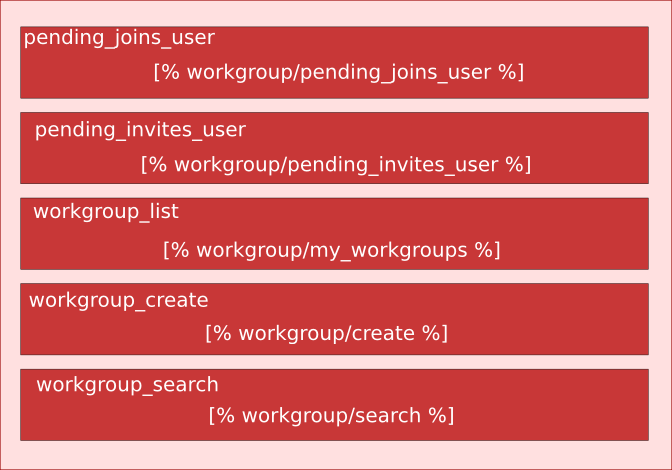
\includegraphics[scale=0.6]{../rome/docs/images/workgroup_page_structure}
\caption{Structure of the Workgroups Page}\label{fig:workgroups_main}
\end{figure}

\paragraph{}
The workgroups controller provides AJAX methods to return the \texttt{pending\_joins} and \texttt{workgroup\_list} div contents. These are used to update the appropriate content when a user's workgroups are changed via an AJAX call. The workgroup list separates workgroups into those of which a user is leader, and those to which they belong. A user may leave a workgroup unless they own it. Workgroups that they own may be deleted and managed. While the delete and leave links trigger AJAX calls to the appropriate controller actions, the manage link returns the management page for the workgroup in question, which allows the user to alter the details of the workgroup in the database, hand ownership of the group to another user, accept or reject membership requests and send out invitations.

